% Define the document type and font size
\documentclass[12pt]{article}

\usepackage[spanish]{babel} % Package for the Spanish language
\usepackage[utf8]{inputenc} % Package for UTF-8 character encoding
\usepackage{geometry} % Package to configure document margins
\usepackage{graphicx} % Package to include graphics
\usepackage{listings} % Package to include source code in the document
\usepackage{xcolor} % Package to define colors
\usepackage{fancyhdr} % Package to customize headers and footers
\usepackage{amsmath} % Package for advanced mathematical symbols and environments
\usepackage{amssymb} % Package for additional mathematical symbols
\usepackage[hidelinks]{hyperref} % Package for hyperlinks in index and references (Keep this as the last package loaded)

\setlength{\parskip}{1em} % Space between paragraphs
\setlength{\parindent}{0.0in} % Indentation for paragraphs

% Definition of colors for source code
\definecolor{COLOR_COMMENTS}{HTML}{999999}
\definecolor{COLOR_KEYWORDS}{HTML}{37a5a6}
\definecolor{COLOR_IDENTIFIERS}{HTML}{ea76cb}
\definecolor{COLOR_STRINGS}{HTML}{ff7858}

% Configuration of the listings environment to display source code
\lstset{
frame=shadowbox,
aboveskip=3mm,
belowskip=3mm,
xleftmargin=10mm,
xrightmargin=10mm,
showstringspaces=false,
columns=flexible,
basicstyle={\footnotesize\ttfamily},
numbers=left,
numberstyle=\tiny\color{COLOR_COMMENTS},
keywordstyle=\color{COLOR_KEYWORDS},
stringstyle=\color{COLOR_STRINGS},
commentstyle=\color{COLOR_COMMENTS},
breaklines=true,
breakatwhitespace=true,
tabsize=4,
}

% Configuration of document margins
\geometry{
    a4paper,
    left=25mm,
    right=25mm,
    top=25mm,
    bottom=25mm
}
\graphicspath{{../img}} % Path for images

\title{Simulación de Distribución de Calor en 2D} % Document title
\author{María Laura Reina y Victoria Ruza} % Document author
\date{\today} % Document date

\begin{document}

    \begin{titlepage}
        \centering
        {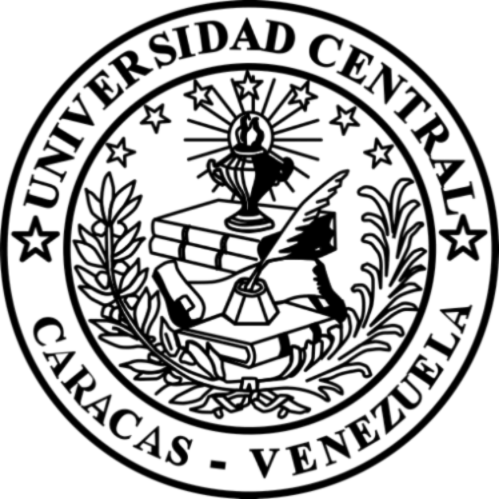
\includegraphics[width=0.2\textwidth]{logoBlack}\par}
        {\large {Universidad Central de Venezuela}\par}
        {\large {Facultad de Ciencias}\par}
        {\large {Escuela de Computación}\par}
        {\large {Cálculo Científico}\par}
        \vfill
        {\Huge {Simulación de Distribución de Calor en 2D}\par}
        \vfill
        {\large María Laura Reina y Victoria Ruza\par}
        \vspace{0.5cm}
        {\large \today\par}
    \end{titlepage}

    \pagenumbering{gobble}
    \tableofcontents
    \newpage
    \pagenumbering{arabic}

    \section{Objetivos}
        \subsection{Objetivo General}
            Simular la distribución de calor en una placa bidimensional utilizando el método de diferencias finitas.
        \subsection{Objetivos Específicos}
            \begin{itemize}
                \item Implementar el método de diferencias finitas para resolver la ecuación de Poisson en 2D.
                \item Analizar la influencia de una fuente de calor puntual en la distribución térmica.
                \item Comparar los resultados obtenidos con y sin la presencia de la fuente de calor para entender su impacto en el sistema.
                \item Visualizar la distribución de temperatura mediante mapas de calor para interpretar los resultados de manera gráfica.
            \end{itemize}
    \newpage

    \section{Introducción}
    El modelado de la distribución de temperatura sobre una placa homogénea bidimensional se rige por la ecuación diferencial parcial (EDP) de Poisson:
    \begin{equation}
    \frac{\partial^2 u}{\partial x^2} + \frac{\partial^2 u}{\partial y^2} = f(x,y)
    \end{equation}
    Donde $u(x,y)$ representa la temperatura en una coordenada espacial continua y $f(x,y)$ modela la densidad de fuentes de calor internas. En ausencia de fuentes ($f(x,y) = 0$), la expresión se reduce a la ecuación elíptica de Laplace. 

    Dado que las soluciones analíticas directas están limitadas a geometrías y condiciones ideales, este trabajo implementa el Método de Diferencias Finitas (MDF) para aproximar la solución sobre una placa cuadrada $[0,1] \times [0,1]$ sujeta a condiciones de frontera fijas (Dirichlet).

    \section{Metodología Numérica y Discretización}

    \subsection{Aproximación por Diferencias Centradas}
    Para transformar este problema continuo en un problema puramente algebraico, se discretiza el dominio espacial mediante una malla uniforme de paso $h = \frac{1}{n+1}$, donde $n=20$ es el número de nodos internos por dimensión, acumulando un total de $n^2 = 400$ incógnitas.

    Aproximando las segundas derivadas parciales mediante diferencias finitas centradas de segundo orden (cuyo error de truncamiento es $\mathcal{O}(h^2)$) se obtiene:
    \begin{equation}
    \frac{\partial^2 u}{\partial x^2} \approx \frac{u_{i+1,j} - 2u_{i,j} + u_{i-1,j}}{h^2}, \quad \frac{\partial^2 u}{\partial y^2} \approx \frac{u_{i,j+1} - 2u_{i,j} + u_{i,j-1}}{h^2}
    \end{equation}

    Sustituyendo estas aproximaciones algebraicas en la ecuación de Poisson y multiplicando la expresión por $-h^2$ para evitar operaciones fraccionarias en el ensamblaje de la matriz, se deriva el balance energético discreto por nodo:
    \begin{equation}
    4u_{i,j} - (u_{i+1,j} + u_{i-1,j} + u_{i,j+1} + u_{i,j-1}) = h^2 f_{i,j}
    \end{equation}

    \subsection{Mapeo de Índices y Condiciones de Frontera}
    El sistema lineal global toma la forma general $Au = b$. Como las incógnitas físicas se encuentran indexadas en un espacio bidimensional $(i, j)$, se implementa un mapeo biyectivo por filas para aplanar la malla hacia un vector unidimensional $u \in \mathbb{R}^{400}$ mediante la función de indexación $k = i \cdot n + j$.

    Las condiciones de frontera impuestas por el enunciado corresponden a temperaturas fijas en los bordes de la placa, representando fuentes térmicas constantes. Específicamente, se asignan los siguientes valores:
    \begin{itemize}
        \item Borde Superior ($y=1$): $100^\circ\text{C}$
        \item Borde Inferior ($y=0$): $0^\circ\text{C}$
        \item Bordes Laterales (Izquierda $x=0$, Derecha $x=1$): $50^\circ\text{C}$
    \end{itemize}

    Dado que los nodos frontera poseen valores deterministas conocidos, no forman parte de las variables del sistema. Cuando un nodo adyacente a la celda analizada coincide con un límite del dominio, su valor constante es removido de la parte izquierda de la ecuación y es trasladado de manera acumulativa hacia el vector de carga (lado derecho de la igualdad, $b_k$).
    \subsection{Optimización Mediante Almacenamiento Disperso}
    Considerando que cada fila del sistema interactúa únicamente con un máximo de 4 vecinos geométricos adyacentes y su propia diagonal, la matriz del sistema $A \in \mathbb{R}^{400 \times 400}$ está compuesta de forma abrumadora por elementos nulos. Almacenar esta matriz en un formato denso tradicional penaliza severamente el uso de memoria. Por ende, se recurre a la abstracción de matrices dispersas de la librería \texttt{scipy.sparse} (formato \texttt{csr\_matrix}), optimizando la resolución del sistema lineal mediante el solucionador directo \texttt{spsolve}.

    \section{Análisis de Resultados}

    \subsection{Estructura y Patrón de Bandas de la Matriz $A$}
    El patrón de esparcimiento espacial de los coeficientes no nulos en la matriz $A$ se visualiza mediante un gráfico de dispersión instrumental.

    \begin{figure}[htbp]
        \centering
        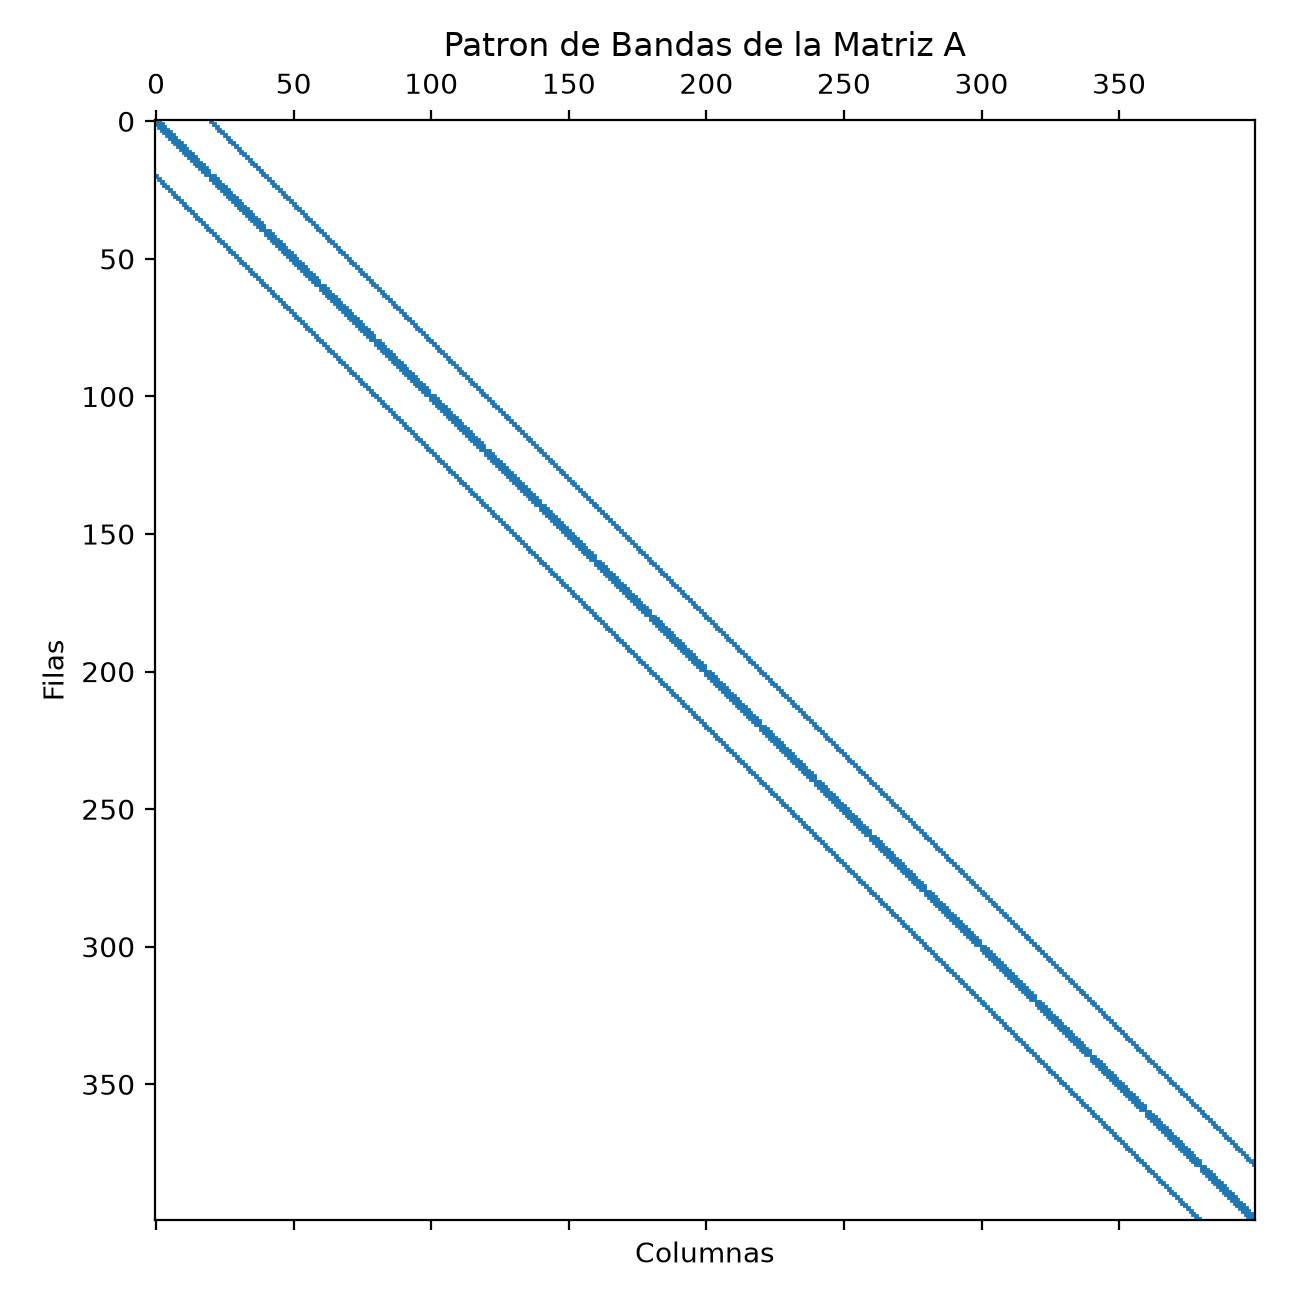
\includegraphics[width=0.5\textwidth]{01_patron_bandas_matriz_A.png}
        \caption{Gráfico de dispersión que evidencia la naturaleza dispersa y estructurada en bandas de la matriz $A$.}
        \label{fig:spy}
    \end{figure}

    En la siguiente figura se observa que, la matriz exhibe una diagonal principal dominante bien definida en conjunto con cuatro diagonales secundarias adyacentes de carácter simétrico. Los elementos de la diagonal principal poseen el coeficiente algebraico constante $A[k,k] = 4$, reflejando la auto-resistencia e interdependencia del nodo sobre sí mismo. Las subdiagonales simétricas reflejan las interacciones locales con coeficientes $-1$ hacia los vecinos espaciales. El distanciamiento constante observado en las bandas más externas corresponde exactamente al salto indexado necesario para saltar a la fila adyacente superior o inferior dentro de la estructura unidimensional aplanada ($k \pm n$).

    \subsection{Distribución de Temperatura con Fuente de Calor}
    La siguiente figura expone la distribución bidimensional de temperatura definitiva sobre la superficie total de la placa (habiendo reincorporado los marcos físicos de las fronteras), correlacionando un mapa de color indexado y curvas de nivel isotérmicas.

    \begin{figure}[htbp]
        \centering
        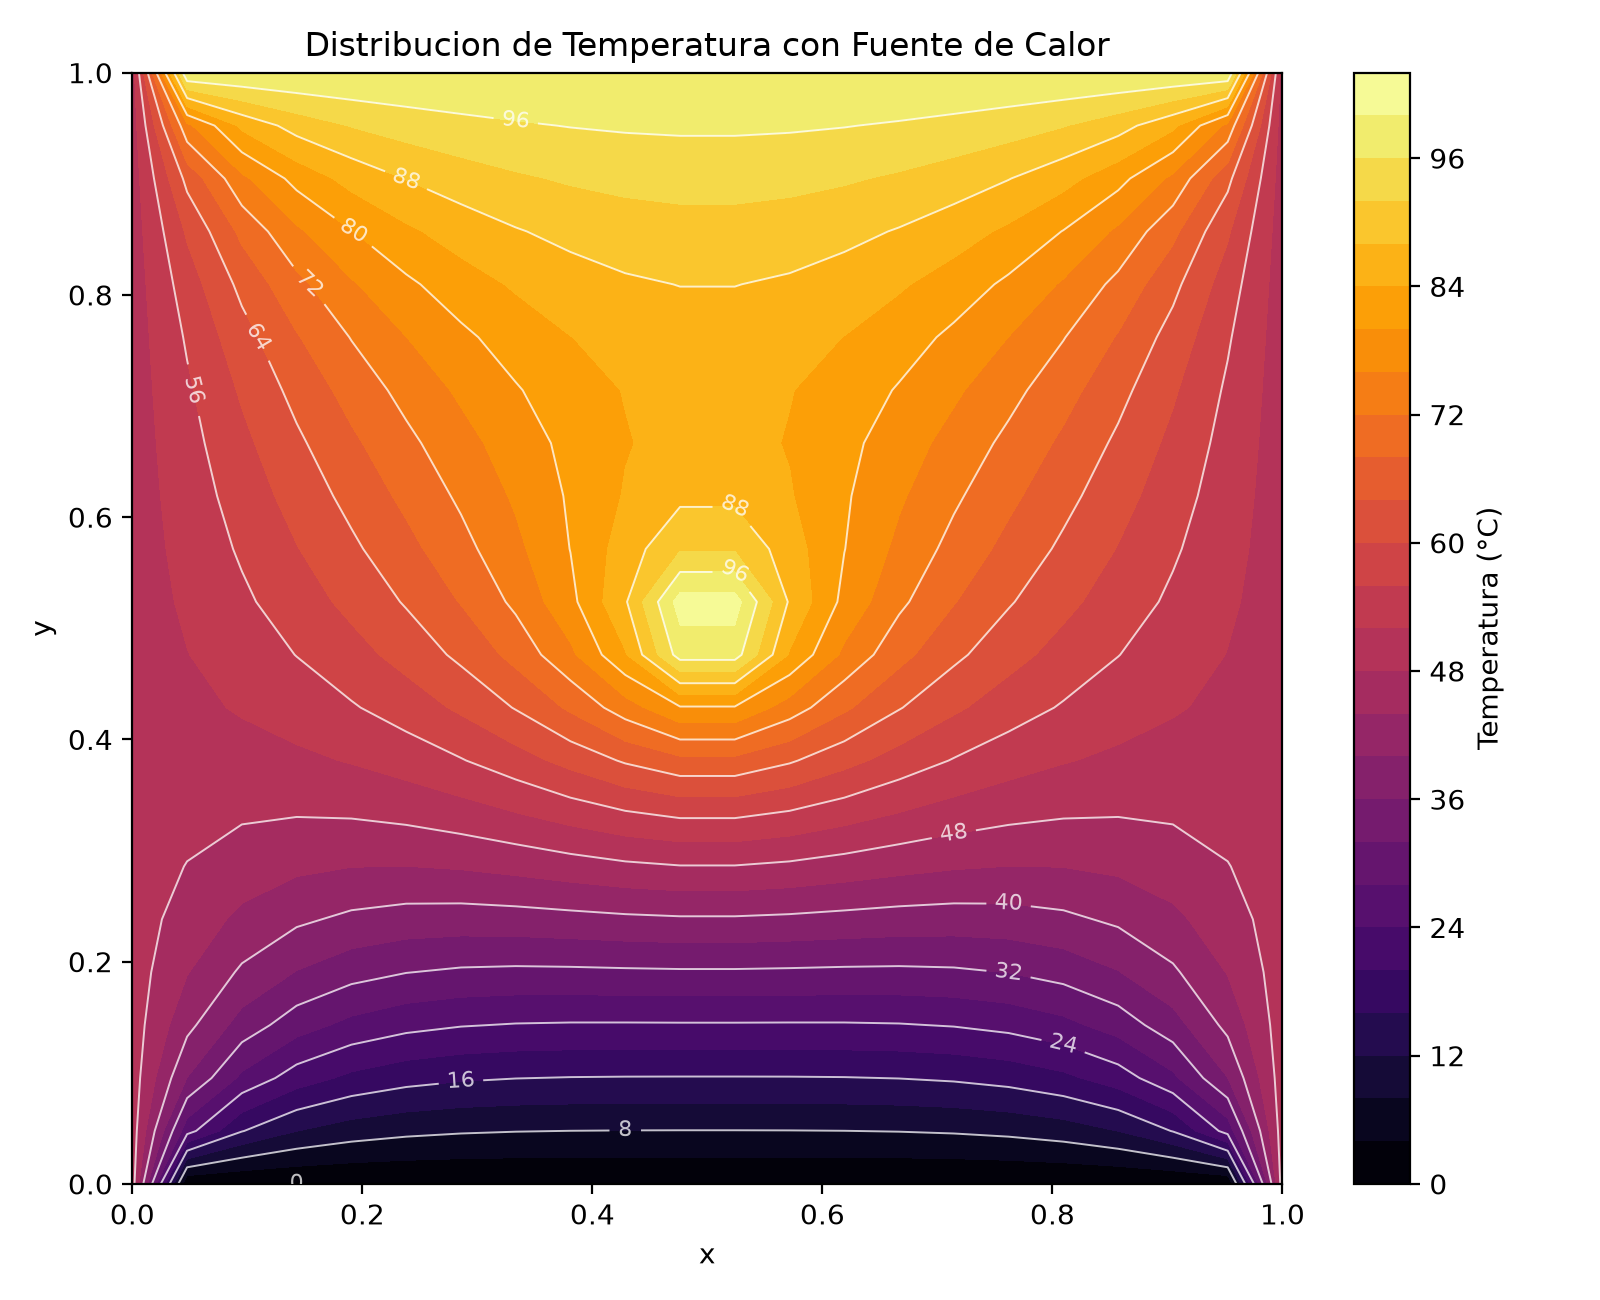
\includegraphics[width=0.6\textwidth]{02_heatmap_con_isotermas.png}
        \caption{Mapa de calor con líneas isotermas superpuestas bajo la influencia de una fuente de calor central.}
        \label{fig:heatmap}
    \end{figure}

    Las isotermas representan trayectorias geométricas donde el potencial térmico es idéntico. En la vecindad de los bordes laterales e inferiores, el calor decae de forma monótona, condicionado por los sumideros de $50^\circ\text{C}$ y $0^\circ\text{C}$. Sin embargo, la imposición de una fuente puntual hiper-intensa en las coordenadas del centro físico genera una deformación geométrica radical. Las curvas concéntricas distribuidas alrededor del punto central evidencian un comportamiento de disipación radial hacia el exterior, con un gradiente térmico extremadamente pronunciado. La presencia de esta fuente de calor focalizada induce un fenómeno de saturación térmica que se extiende hacia los bordes adyacentes, alterando significativamente la distribución de temperatura en toda la región central de la placa.

    \subsection{Análisis Comparativo Físico (Presencia vs. Ausencia de Fuente)}
    A fin de categorizar el impacto de la fuente puntual, se contrastan los mapas de calor para ambos escenarios: el estado libre de fuentes y el estado perturbado.

    \begin{figure}[htbp]
        \centering
        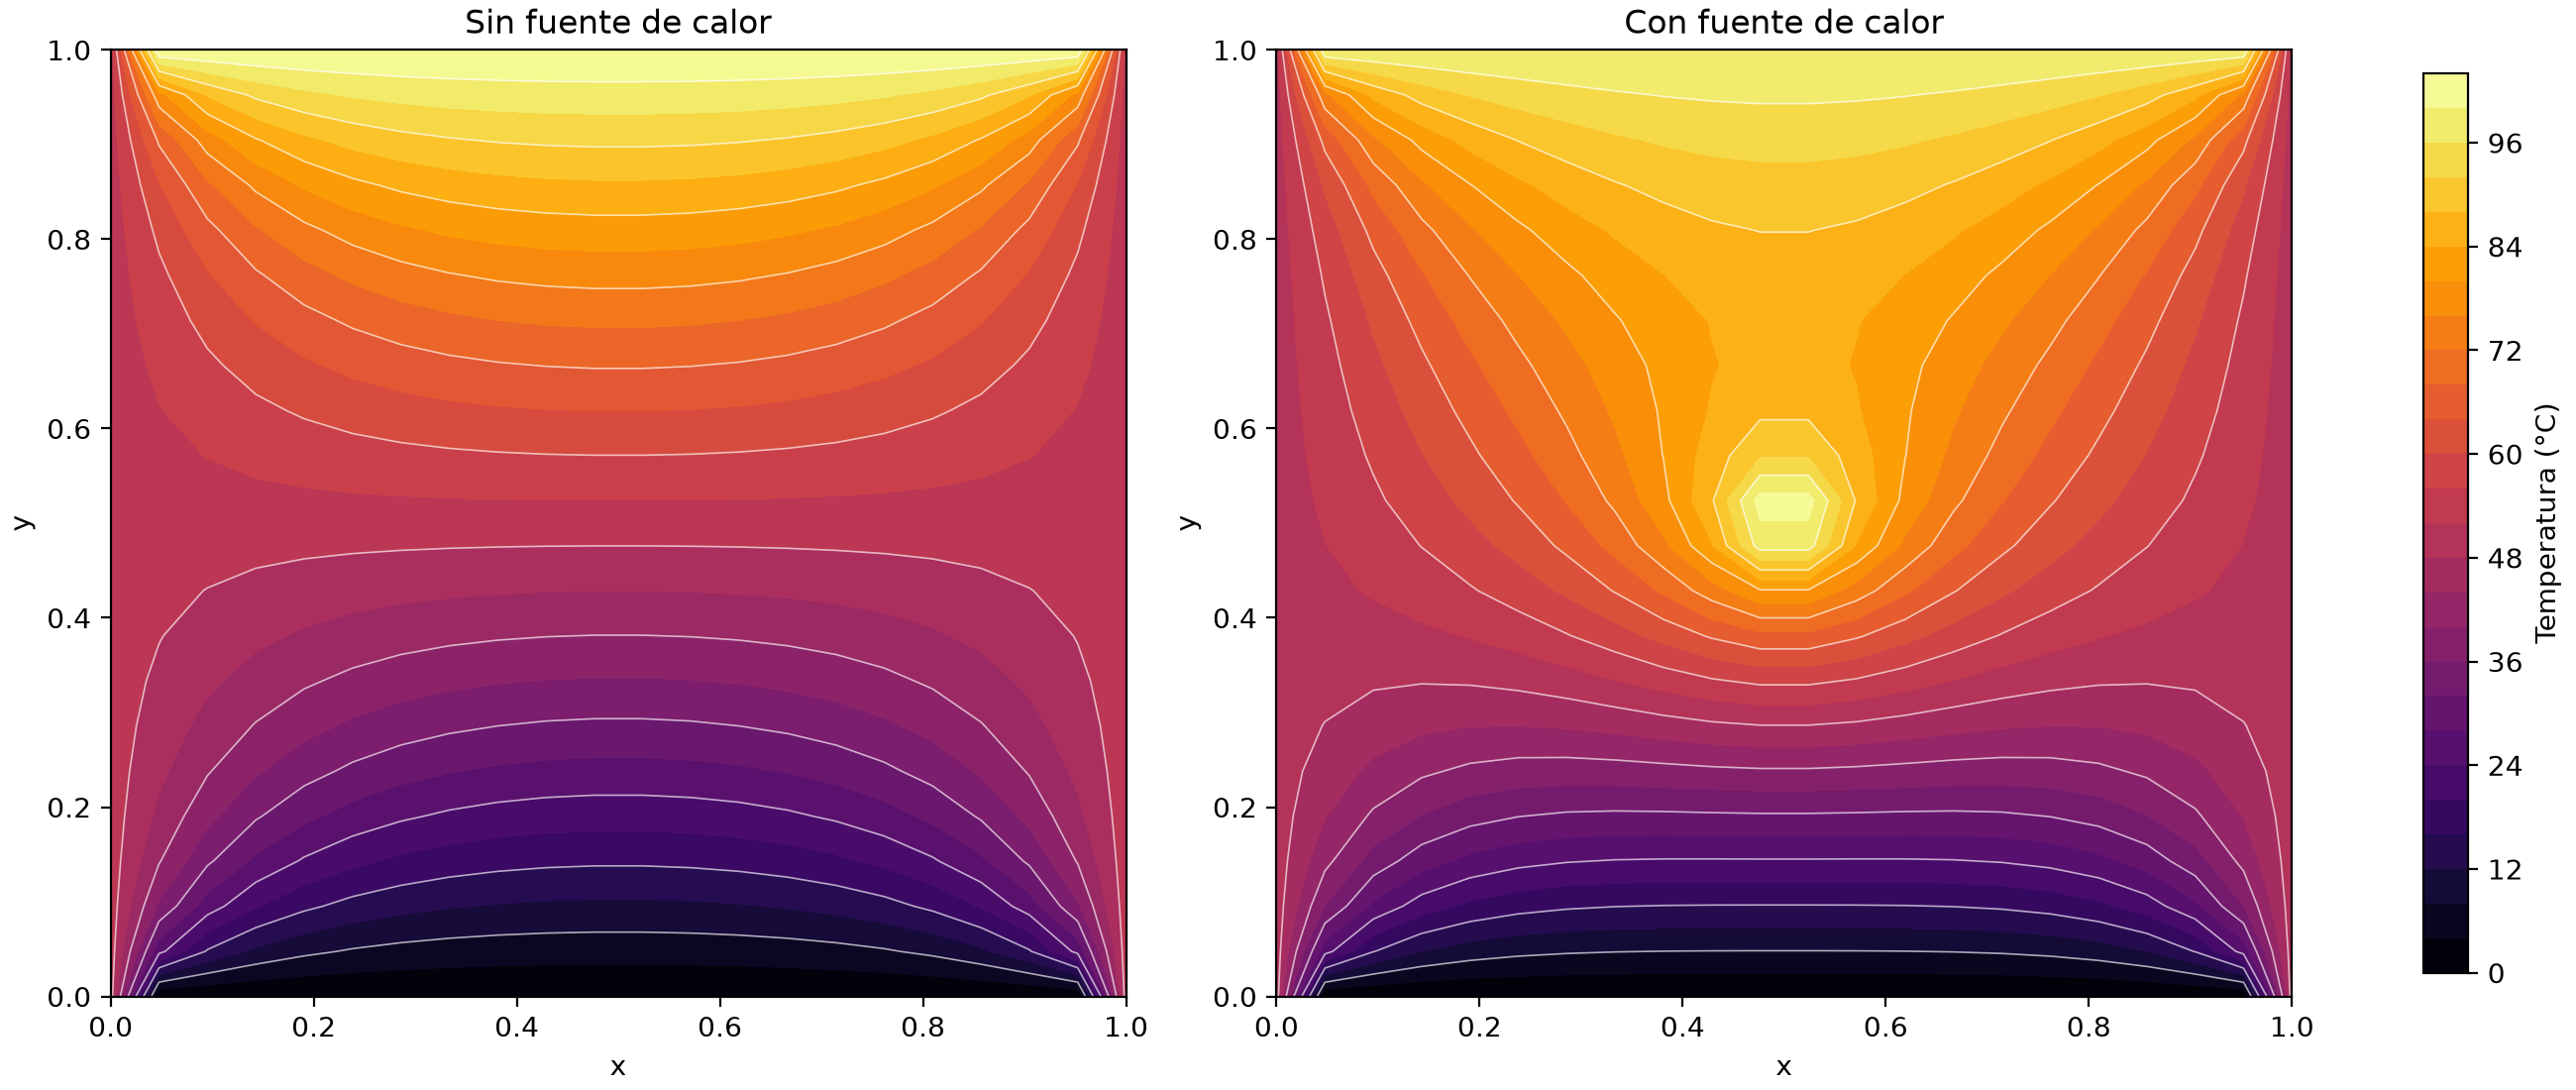
\includegraphics[width=0.9\textwidth]{03_comparacion_con_y_sin_fuente.png}
        \caption{Comparación visual del comportamiento térmico de la placa: Estado Libre de Fuentes (Izquierda) vs. Estado Perturbado (Derecha).}
        \label{fig:comparativa}
    \end{figure}

    El análisis comparativo de ambos estados operacionales demuestra los siguientes fenómenos físicos:
    \begin{itemize}
        \item \textbf{Configuración sin fuente:} El flujo térmico se desplaza en condiciones de simetría pura desde el borde superior caliente hacia el borde inferior, mostrando un decremento de temperatura uniforme y predecible.
        \item \textbf{Configuración con fuente:} La introducción de la fuente de carga focalizada en el centro actúa como un nodo de inyección masiva de energía. El calor inyectado excede los límites impuestos por las fronteras, forzando una redistribución no homogénea del campo térmico en toda la región central de la placa.
    \end{itemize}

    \subsection{Análisis del Perfil Transversal Central}
    Para cuantificar con precisión matemática la severidad de la perturbación focalizada, se efectúa un corte transversal horizontal intermedio evaluando la función discreta de la temperatura a lo largo del segmento lineal $u(x, 0.5)$, representado en la Figura 4.

    \begin{figure}[htbp]
        \centering
        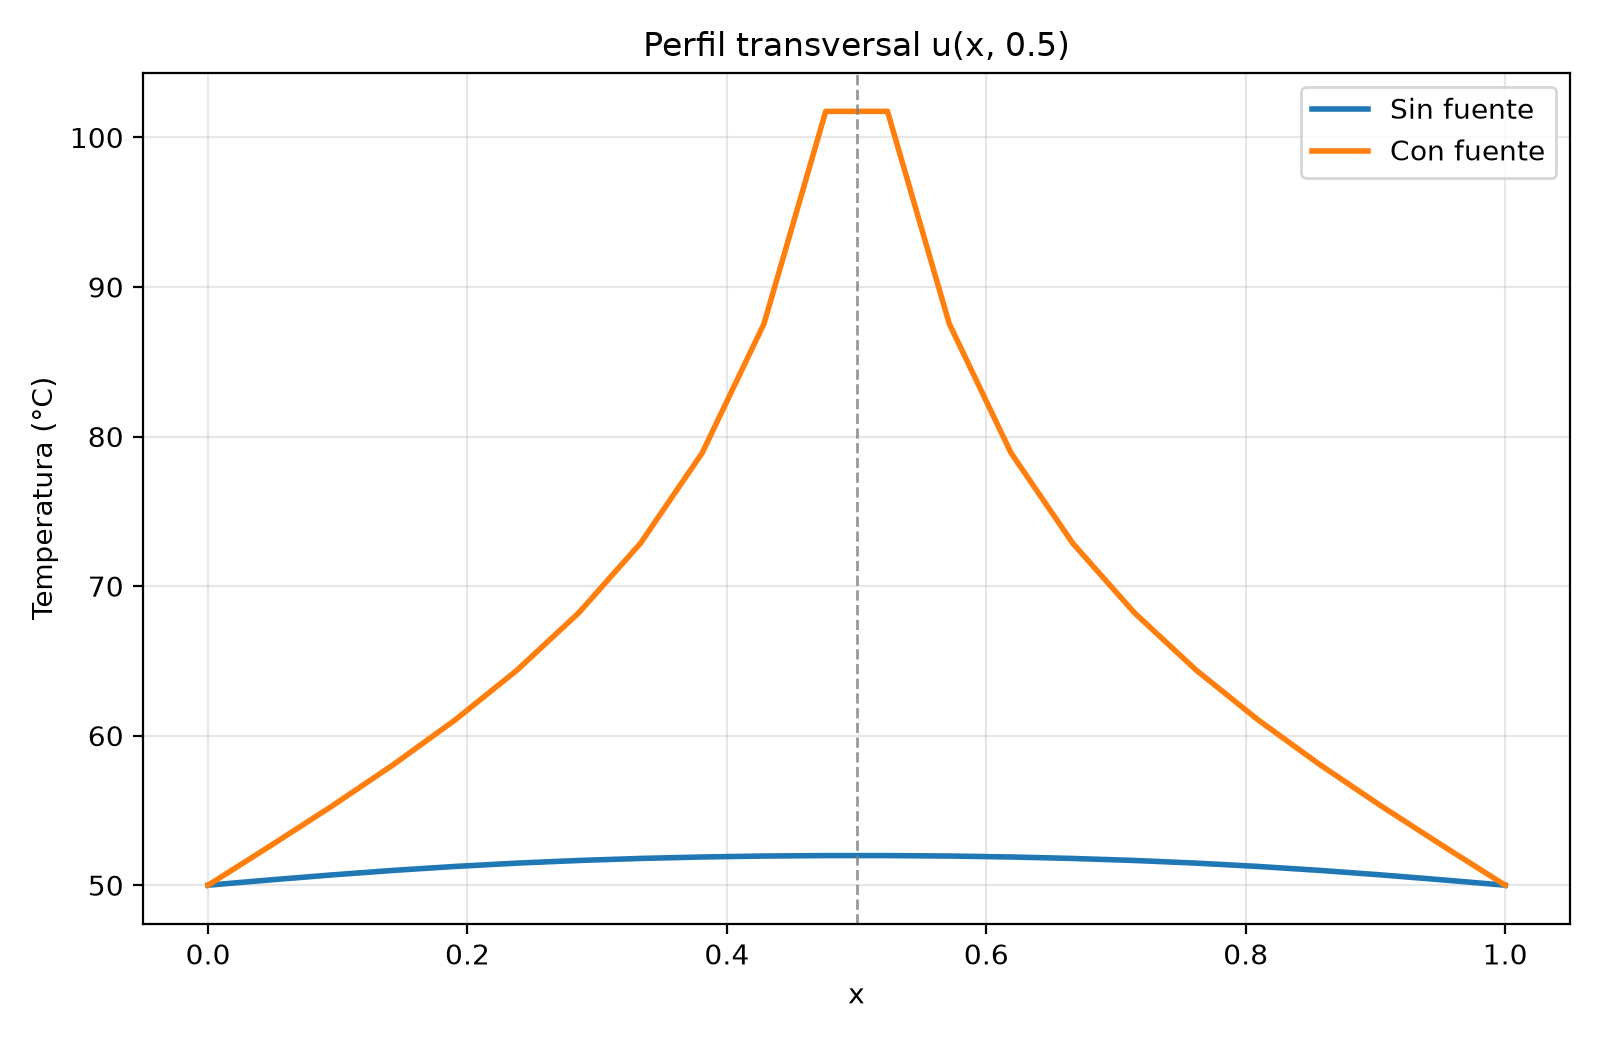
\includegraphics[width=0.65\textwidth]{04_perfil_transversal_central.png}
        \caption{Variación de la temperatura a lo largo de la sección transversal horizontal central $y=0.5$.}
        \label{fig:perfil}
    \end{figure}

    La observación analítica de las curvas revela un comportamiento contrastante de alta relevancia diagnóstica. En el escenario sin fuente de calor (línea azul), el perfil manifiesta una geometría parabólica suave y simétrica, que inicia en el valor de frontera $50^\circ\text{C}$ ($x=0$), alcanza un máximo leve y sutil en el punto medio debido a la conducción difusiva descendente, y converge nuevamente en $50^\circ\text{C}$ ($x=1$). 

    Por el contrario, el escenario con presencia de fuente (línea naranja) exhibe una discontinuidad manifestada justo en el entorno del centro geométrico ($x=0.5$), proyectando un incremento abrupto y empinado de temperatura que roza los $102^\circ\text{C}$. Este pico local es un claro indicador de la influencia dominante de la fuente puntual, superando incluso el valor máximo impuesto por el borde superior. La forma simétrica y pronunciada del perfil en este caso refleja la naturaleza no homogénea de la ecuación o la alta localización espacial de la respuesta térmica ante perturbaciones focalizadas, evidenciando un fenómeno de saturación térmica que se extiende hacia los bordes adyacentes.

    \newpage
    \section{Referencias}
    \begin{itemize}
        \item Stewart Math, “Ecuación del calor | Ecuaciones Diferenciales Parciales,” YouTube. Aug. 23, 2023. [Online]. Available:\newline \url{https://www.youtube.com/watch?v=Swk5OPyu-cI}.
        \item Stewart Math, “Ecuación de Laplace | Ecuaciones Diferenciales Parciales,” YouTube. Sep. 18, 2024. [Online]. Available:\newline \url{https://www.youtube.com/watch?v=gMTydl83r2M}.
        \item cctmexico, “Método de Diferencias Finitas | Ecuaciones Diferenciales |Métodos Numéricos,” YouTube. Apr. 25, 2020. [Online]. Available:\newline \url{https://www.youtube.com/watch?v=KZpHx9ZJ0wY}.
        \item Aerodynamic CFD, “Finite Difference for 2D Poisson’s equation,” YouTube. Sep. 24, 2018. [Online]. Available:\newline \url{https://www.youtube.com/watch?v=ytnKP1pbJTg}.
    \end{itemize}
\end{document}